\documentclass{article}

% ============================================================
% PACKAGES
% ============================================================

\usepackage{amsmath}
\usepackage{amssymb}
\usepackage{geometry}
\usepackage{tikz}
\usepackage{pgfplots}
\usepackage{array}

\geometry{margin=1in}
\pgfplotsset{compat=1.18}

% ============================================================
% DOCUMENT INFORMATION
% ============================================================

\title{APM1220: Applied Multivariate Data Analysis}
\author{Kristen Jelaena Cesista}
\date{August 2026}

\begin{document}

% ============================================================
% TITLE
% ============================================================

\noindent
\textbf{APM1220: Applied Multivariate Data Analysis}\\
\textbf{FA 2. Sample Geometry and Random Sampling}

\vspace{0.5cm}

\noindent
\textbf{Total: 40 Points}

\vspace{0.5cm}

\noindent
\textbf{Instructions:}

\begin{itemize}
    \item Answer all questions completely and show all necessary steps,
    intermediate calculations, and mathematical proofs clearly to receive
    full credit.

    \item Where matrix operations are required, ensure that dimensions
    conform before performing any matrix multiplications, additions, or
    inversions.

    \item Present all final matrix entries and numerical results in exact,
    simplified form (e.g., fractions or radicals) unless decimals are
    specifically requested.

    \item Clearly label final answers for each sub-problem (a, b, c, etc.).
\end{itemize}

\vspace{0.5cm}

% ============================================================
% PROBLEM 3.1
% ============================================================

\noindent
{\Large \textbf{Problem 3.1}}
\hfill
{\large \textbf{(8 points)}}

\vspace{0.3cm}

\noindent
\textbf{Question:} Given the data matrix

$$
X =
\begin{bmatrix}
9 & 1\\
5 & 3\\
1 & 2
\end{bmatrix},
$$

\noindent
\textbf{(a)} Graph the scatter plot in $p=2$ dimensions. Locate the
sample mean on your diagram.

\vspace{0.2cm}

\noindent
\textbf{(b)} Sketch the $n=3$-dimensional representation of the data,
and plot the deviation vectors $y_1-\bar{x}_1\mathbf{1}$ and
$y_2-\bar{x}_2\mathbf{1}$.

\vspace{0.2cm}

\noindent
\textbf{(c)} Sketch the deviation vectors in (b) emanating from the
origin. Calculate the lengths of these vectors and the cosine of the
angle between them. Relate these quantities to $S_n$ and $R$.

\vspace{0.5cm}

% ------------------------------------------------------------
% PART A
% ------------------------------------------------------------

\subsection*{(a)}

To graph the scatter plot in $p=2$ dimensions, we first identify the
points, which are

$$
(9,1),\qquad (5,3),\qquad (1,2).
$$

Afterwards the sample mean vector should be calculated:

$$
\bar{x}
=
\begin{bmatrix}
(9+5+1)/3\\
(1+3+2)/3
\end{bmatrix}
=
\begin{bmatrix}
5\\
2
\end{bmatrix}.
$$

Therefore,

$$
\boxed{
\text{The sample mean is }
\bar{x}
=
\begin{bmatrix}
5\\
2
\end{bmatrix}}
$$

\vspace{0.5cm}

\begin{center}
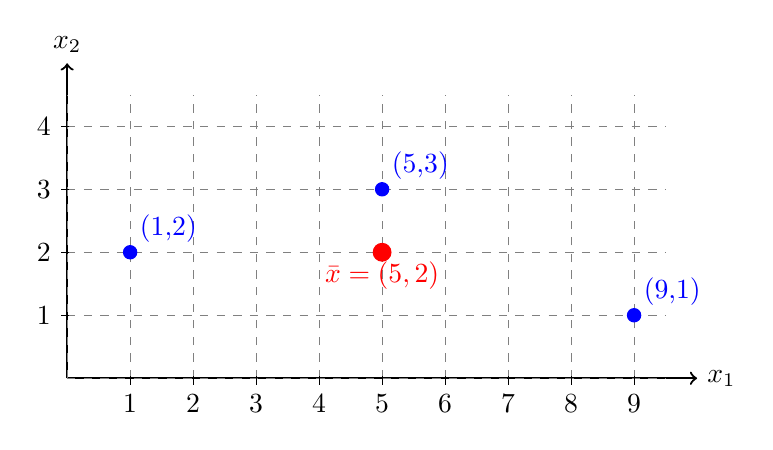
\begin{tikzpicture}[scale=0.8]

    % Draw axes
    \draw[->, thick] (0,0) -- (10,0) node[right] {$x_1$};
    \draw[->, thick] (0,0) -- (0,5) node[above] {$x_2$};

    % Draw grid & ticks
    \draw[step=1cm,gray,very thin,dashed] (0,0) grid (9.5,4.5);

    \foreach \x in {1,...,9}
        \draw (\x,1pt) -- (\x,-3pt)
        node[anchor=north] {\x};

    \foreach \y in {1,...,4}
        \draw (1pt,\y) -- (-3pt,\y)
        node[anchor=east] {\y};

    % Plot data points
    \filldraw[blue] (9,1) circle (3pt)
        node[anchor=south west] {(9,1)};

    \filldraw[blue] (5,3) circle (3pt)
        node[anchor=south west] {(5,3)};

    \filldraw[blue] (1,2) circle (3pt)
        node[anchor=south west] {(1,2)};

    % Plot Mean
    \filldraw[red] (5,2) circle (4pt)
        node[anchor=north] {$\bar{x}=(5,2)$};

\end{tikzpicture}
\end{center}

\vspace{0.3cm}

% ------------------------------------------------------------
% PART B
% ------------------------------------------------------------

\subsection*{(b)}

For the $n=3$-dimensional representation, each variable will be represented
as a vector in $\mathbb{R}^3$.

The two variable vectors are then:

$$
y_1=
\begin{bmatrix}
9\\
5\\
1
\end{bmatrix},
\qquad
y_2=
\begin{bmatrix}
1\\
3\\
2
\end{bmatrix}.
$$

The sample means are

$$
\bar{x}_1=\frac{9+5+1}{3}=5,
\qquad
\bar{x}_2=\frac{1+3+2}{3}2.
$$

The vector of ones is

$$
\mathbf{1}=
\begin{bmatrix}
1\\
1\\
1
\end{bmatrix}.
$$

Computing for the first variable:

$$
y_1-\bar{x}_1\mathbf{1}
=
\begin{bmatrix}
9\\
5\\
1
\end{bmatrix}
-
5
\begin{bmatrix}
1\\
1\\
1
\end{bmatrix}
$$

$$
=
\begin{bmatrix}
9\\
5\\
1
\end{bmatrix}
-
\begin{bmatrix}
5\\
5\\
5
\end{bmatrix}
=
\begin{bmatrix}
4\\
0\\
-4
\end{bmatrix}.
$$

Thus,

$$
\boxed{
y_1-\bar{x}_1\mathbf{1}
=
\begin{bmatrix}
4\\
0\\
-4
\end{bmatrix}}
$$

Computing for the second variable:

$$
y_2-\bar{x}_2\mathbf{1}
=
\begin{bmatrix}
1\\
3\\
2
\end{bmatrix}
-
2
\begin{bmatrix}
1\\
1\\
1
\end{bmatrix}
$$

$$
=
\begin{bmatrix}
1\\
3\\
2
\end{bmatrix}
-
\begin{bmatrix}
2\\
2\\
2
\end{bmatrix}
=
\begin{bmatrix}
-1\\
1\\
0
\end{bmatrix}.
$$

Thus,

$$
\boxed{
y_2-\bar{x}_2\mathbf{1}
=
\begin{bmatrix}
-1\\
1\\
0
\end{bmatrix}}
$$

The mean points in $\mathbb{R}^3$ are

$$
\bar{x}_1\mathbf{1}
=
\begin{bmatrix}
5\\
5\\
5
\end{bmatrix},
\qquad
\bar{x}_2\mathbf{1}
=
\begin{bmatrix}
2\\
2\\
2
\end{bmatrix}.
$$

The deviation vectors which were just  calculated can be used to connect these mean points to $y_1$ and $y_2$.

\vspace{0.3cm}

\begin{center}
\begin{tikzpicture}[scale=0.65]

    % Axes
    \draw[->, thick] (0,0) -- (6,0)
        node[right] {$x_1$};

    \draw[->, thick] (0,0) -- (-3,3)
        node[above left] {$x_2$};

    \draw[->, thick] (0,0) -- (0,-5)
        node[below] {$x_3$};

    % y1 and mean point
    \filldraw[blue] (4,0) circle (3pt)
        node[above right] {$y_1=(9,5,1)$};

    \filldraw[red] (2.2,0) circle (3pt)
        node[below] {$\bar{x}_1\mathbf{1}$};

    % Deviation y1
    \draw[->, thick, blue] (2.2,0) -- (4,0);

    % y2 and mean point
    \filldraw[blue] (-1,1) circle (3pt)
        node[above left] {$y_2=(1,3,2)$};

    \filldraw[red] (-0.7,0.7) circle (3pt)
        node[below left] {$\bar{x}_2\mathbf{1}$};

    % Deviation y2
    \draw[->, thick, blue] (-0.7,0.7) -- (-1,1);

\end{tikzpicture}
\end{center}

% ------------------------------------------------------------
% PART C
% ------------------------------------------------------------

\subsection*{(c)}

Let

$$
d_1=y_1-\bar{x}_1\mathbf{1}
=
\begin{bmatrix}
4\\
0\\
-4
\end{bmatrix}
$$

and

$$
d_2=y_2-\bar{x}_2\mathbf{1}
=
\begin{bmatrix}
-1\\
1\\
0
\end{bmatrix}.
$$

The length of $d_1$ is calculated as:

$$
\begin{aligned}
\|d_1\|
&=
\sqrt{4^2+0^2+(-4)^2}\\
&=
\sqrt{16+16}\\
&=
\sqrt{32}\\
&=
4\sqrt{2}.
\end{aligned}
$$

$$
\boxed{\|d_1\|=4\sqrt{2}}
$$

Meanwhile, the length of $d_2$ is

$$
\begin{aligned}
\|d_2\|
&=
\sqrt{(-1)^2+1^2+0^2}\\
&=
\sqrt{1+1}\\
&=
\sqrt{2}.
\end{aligned}
$$

$$
\boxed{\|d_2\|=\sqrt{2}}
$$

Now we calculate the dot product:

$$
d_1^Td_2
=
\begin{bmatrix}
4&0&-4
\end{bmatrix}
\begin{bmatrix}
-1\\
1\\
0
\end{bmatrix}
$$

$$
=
(4)(-1)+(0)(1)+(-4)(0)
=
-4.
$$

To get the cosine of the angle $\theta$ between the vectors, we will use the following formula:

$$
\cos\theta
=
\frac{d_1^Td_2}
{\|d_1\|\|d_2\|}.
$$

Inserting the values gives us,

$$
\cos\theta
=
\frac{-4}
{(4\sqrt{2})(\sqrt{2})}
=
\frac{-4}{8}
=
-\frac{1}{2}.
$$

$$
\boxed{\cos\theta=-\frac{1}{2}}
$$

Therefore,

$$
\theta
=
\cos^{-1}\left(-\frac{1}{2}\right)
$$

$$
\boxed{\theta=120^\circ}.
$$

The sample covariance matrix using $S_n=\frac{1}{n}D^TD$ is

$$
S_n
=
\frac{1}{3}
\begin{bmatrix}
d_1^Td_1 & d_1^Td_2\\
d_2^Td_1 & d_2^Td_2
\end{bmatrix}.
$$

Since

$$
d_1^Td_1=32,
\qquad
d_1^Td_2=-4,
\qquad
d_2^Td_2=2,
$$

plugging the values in, we get

$$
S_n
=
\frac{1}{3}
\begin{bmatrix}
32&-4\\
-4&2
\end{bmatrix}.
$$

Thus,

$$
\boxed{
S_n=
\begin{bmatrix}
\dfrac{32}{3}&-\dfrac{4}{3}\\[0.5em]
-\dfrac{4}{3}&\dfrac{2}{3}
\end{bmatrix}}
$$

The diagonal elements of $S_n$ are directly related to the squared
lengths of the deviation vectors. Since

$$
S_n=\frac{1}{n}D^TD
$$

with $n=3$, we have

$$
(S_n)_{11}
=
\frac{1}{3}d_1^Td_1
=
\frac{1}{3}\|d_1\|^2.
$$

Since

$$
\|d_1\|^2=(4\sqrt{2})^2=32,
$$

we obtain

$$
(S_n)_{11}
=
\frac{32}{3}.
$$

Similarly,

$$
(S_n)_{22}
=
\frac{1}{3}d_2^Td_2
=
\frac{1}{3}\|d_2\|^2.
$$

Since

$$
\|d_2\|^2=(\sqrt{2})^2=2,
$$

we obtain

$$
(S_n)_{22}
=
\frac{2}{3}.
$$

Therefore, the squared lengths of the deviation vectors are

$$
\boxed{
\|d_1\|^2=d_1^Td_1=32=3(S_n)_{11}
}
$$

and

$$
\boxed{
\|d_2\|^2=d_2^Td_2=2=3(S_n)_{22}
}
$$

Thus, the diagonal elements of $S_n$ represent the squared lengths
of the centered variable vectors divided by $n$.

The correlation matrix is

$$
R=
\begin{bmatrix}
1&R_{12}\\
R_{12}&1
\end{bmatrix},
$$

plugging in the values, we obtain

$$
R_{12}
=
\frac{(S_n)_{12}}
{\sqrt{(S_n)_{11}(S_n)_{22}}}.
$$

Therefore,

$$
R_{12}
=
\frac{-\frac{4}{3}}
{\sqrt{
\left(\frac{32}{3}\right)
\left(\frac{2}{3}\right)
}}
=
\frac{-\frac{4}{3}}{\frac{8}{3}}
=
-\frac{1}{2}.
$$

Hence,

$$
\boxed{
R=
\begin{bmatrix}
1&-\dfrac12\\
-\dfrac12&1
\end{bmatrix}}
$$

Notice that,

$$
\boxed{R_{12}=\cos\theta=-\frac12}.
$$

Thus, it can be said that the correlation is equal to the cosine of
the angle between the two centered variable vectors.

\vspace{0.3cm}

\begin{center}
\fbox{
\parbox{0.92\textwidth}{
\textbf{The squared lengths are proportional to the value of the sample variances $S_N$, meanwhile the angle in between the two deviation vectors is equal to the sample correlation coefficient $R$}
}
}
\end{center}

% ============================================================
% PROBLEM 3.6
% ============================================================

\newpage

\noindent
{\Large \textbf{Problem 3.6}}
\hfill
{\large \textbf{(8 points)}}

\vspace{0.3cm}

\noindent
\textbf{Question:} Consider the data matrix

$$
X=
\begin{bmatrix}
-1&3&-2\\
2&4&2\\
5&2&3
\end{bmatrix}.
$$

\vspace{0.2cm}

\noindent
\textbf{(a)} Calculate the matrix of deviations (residuals),
$X-\mathbf{1}\bar{x}'$. Is this matrix of full rank? Explain.

\vspace{0.2cm}

\noindent
\textbf{(b)} Determine $S$ and calculate the generalized sample
variance $|S|$. Interpret the latter geometrically.

\vspace{0.2cm}

\noindent
\textbf{(c)} Using the results in (b), calculate the total sample
variance. [See (3-23).]

\vspace{0.5cm}

% ------------------------------------------------------------
% PART A
% ------------------------------------------------------------

\subsection*{(a)}

First we will need to calculate the sample mean vector.

$$
\bar{x}
=
\begin{bmatrix}
(-1+2+5)/3\\
(3+4+2)/3\\
(-2+2+3)/3
\end{bmatrix}
=
\begin{bmatrix}
(6)/3\\
(9)/3\\
(3)/3
\end{bmatrix}
=
\begin{bmatrix}
2\\
3\\
1
\end{bmatrix}.
$$

Thus,

$$
\bar{x}'
=
\begin{bmatrix}
2&3&1
\end{bmatrix}.
$$

The matrix $\mathbf{1}\bar{x}'$ is:

$$
\mathbf{1}\bar{x}'
=
\begin{bmatrix}
1\\
1\\
1
\end{bmatrix}
\begin{bmatrix}
2&3&1
\end{bmatrix}
=
\begin{bmatrix}
2&3&1\\
2&3&1\\
2&3&1
\end{bmatrix}.
$$

Therefore,

$$
X-\mathbf{1}\bar{x}'
=
\begin{bmatrix}
-1&3&-2\\
2&4&2\\
5&2&3
\end{bmatrix}
-
\begin{bmatrix}
2&3&1\\
2&3&1\\
2&3&1
\end{bmatrix}.
$$

$$
\boxed{
X-\mathbf{1}\bar{x}'
=
\begin{bmatrix}
-3&0&-3\\
0&1&1\\
3&-1&2
\end{bmatrix}}
$$

Since this is a square matrix, we can calculate its determinant to see if it's full rank.

$$
\det
\begin{bmatrix}
-3&0&-3\\
0&1&1\\
3&-1&2
\end{bmatrix}
$$

$$
=
(-3)
\begin{vmatrix}
1&1\\
-1&2
\end{vmatrix}
-
(0)
\begin{vmatrix}
0&1\\
3&2
\end{vmatrix}
+
(-3)
\begin{vmatrix}
0&1\\
3&-1
\end{vmatrix}.
$$

$$
=
(-3)\left[(1)(2)-(1)(-1)\right]
-
(0)\left[(0)(2)-(1)(3)\right]
+
(-3)\left[(0)(-1)-(1)(3)\right].
$$

Simplifying,

$$
=
(-3)(2+1)
-
0
+
(-3)(0-3).
$$

$$
=
(-3)(3)+(-3)(-3)
$$

$$
=
-9+9
$$

$$
=0.
$$

$$
\boxed{
\det
\begin{bmatrix}
-3&0&-3\\
0&1&1\\
3&-1&2
\end{bmatrix}
=0
}.
$$

\begin{center}
\fbox{
\parbox{0.88\textwidth}{
\textbf{Since the determinant of the square matrix is zero, the matrix does not have full rank.}
}
}
\end{center}

This occurs because the matrix is mean-centered, meaning at least one row is predictable which goes contradicts the definition of full rank matrix which are matrices of which all rows provide independent information.

% ------------------------------------------------------------
% PART B
% ------------------------------------------------------------

\subsection*{(b)}

The sample covariance matrix is

$$
S=
\frac{1}{n-1}
(X-\mathbf{1}\bar{x}')
(X-\mathbf{1}\bar{x}')'.
$$

Since $n=3$,

$$
S =
\frac{1}{2}
\begin{bmatrix}
-3 & 0 & 3 \\
0 & 1 & -1 \\
-3 & 1 & 2
\end{bmatrix}
\begin{bmatrix}
-3 & 0 & -3 \\
0 & 1 & 1 \\
3 & -1 & 2
\end{bmatrix}
$$

\noindent
To multiply the matrices, we will take the dot product of each row of the first
matrix with each column of the second matrix.

\vspace{0.2cm}

\noindent
\textbf{For the $(1,1)$ entry:}

$$
(-3)(-3) + (0)(0) + (3)(3)
=
9 + 0 + 9
=
18
$$

\noindent
\textbf{For the $(1,2)$ entry:}

$$
(-3)(0) + (0)(1) + (3)(-1)
=
0 + 0 - 3
=
-3
$$

\noindent
\textbf{For the $(1,3)$ entry:}

$$
(-3)(-3) + (0)(1) + (3)(2)
=
9 + 0 + 6
=
15
$$

\noindent
\textbf{For the $(2,1)$ entry:}

$$
(0)(-3) + (1)(0) + (-1)(3)
=
0 + 0 - 3
=
-3
$$

\noindent
\textbf{For the $(2,2)$ entry:}

$$
(0)(0) + (1)(1) + (-1)(-1)
=
0 + 1 + 1
=
2
$$

\noindent
\textbf{For the $(2,3)$ entry:}

$$
(0)(-3) + (1)(1) + (-1)(2)
=
0 + 1 - 2
=
-1
$$

\noindent
\textbf{For the $(3,1)$ entry:}

$$
(-3)(-3) + (1)(0) + (2)(3)
=
9 + 0 + 6
=
15
$$

\noindent
\textbf{For the $(3,2)$ entry:}

$$
(-3)(0) + (1)(1) + (2)(-1)
=
0 + 1 - 2
=
-1
$$

\noindent
\textbf{For the $(3,3)$ entry:}

$$
(-3)(-3) + (1)(1) + (2)(2)
=
9 + 1 + 4
=
14
$$

\noindent
Before multiplying by $\frac{1}{2}$, the matrix product is

$$
\begin{bmatrix}
18 & -3 & 15 \\
-3 & 2 & -1 \\
15 & -1 & 14
\end{bmatrix}.
$$

\noindent
Now multiply every element by $\frac{1}{2}$:

$$
S =
\frac{1}{2}
\begin{bmatrix}
18 & -3 & 15 \\
-3 & 2 & -1 \\
15 & -1 & 14
\end{bmatrix}
$$

$$
\boxed{
S=
\begin{bmatrix}
9&-\dfrac32&-\dfrac{15}{2}\\[0.5em]
-\dfrac32&1&\dfrac12\\[0.5em]
-\dfrac{15}{2}&\dfrac12&7
\end{bmatrix}}
$$

The generalized sample variance is

$$
|S|=\det(S).
$$

Thus,

$$
|S|= 9(7 - 0.25) - (-1.5)(-10.5 - (-3.75)) + 7.5(0.75 - 7.5) = 60.75 - 10.125 - 50.625 = 0.
$$

Therefore,

$$
\boxed{|S|=0}.
$$

Geometrically, the generalized variance represents the squared
volume of the ellipsoid determined by the covariance matrix.
Since $|S|=0$, this volume is zero. This means that the data are linearly dependent and lies in a lower-dimensional hyperplan such as 2D plane.

% ------------------------------------------------------------
% PART C
% ------------------------------------------------------------

\subsection*{(c)}

The total sample variance is the the trace of $S$ which is the sum of the diagonal elements of
$S$:

$$
\operatorname{tr}(S)
=
S_{11}+S_{22}+S_{33}.
$$

$$
\operatorname{tr}(S)
=
9+1+7
=
17.
$$

$$
\boxed{\operatorname{tr}(S)=17}.
$$

% ============================================================
% PROBLEM 3.9
% ============================================================

\newpage

\noindent
{\Large \textbf{Problem 3.9}}
\hfill
{\large \textbf{(8 points)}}

\vspace{0.3cm}

\noindent
\textbf{Question:} The following data matrix contains data on test
scores, with $x_1$ = score on first test, $x_2$ = score on second test,
and $x_3$ = total score on the two tests:

$$
X=
\begin{bmatrix}
12&17&29\\
18&20&38\\
14&16&30\\
20&18&38\\
16&19&35
\end{bmatrix}.
$$

\vspace{0.2cm}

\noindent
\textbf{(a)} Obtain the mean corrected data matrix, and verify that the
columns are linearly dependent. Specify an $a'=[a_1,a_2,a_3]$ vector
that establishes the linear dependence.

\vspace{0.2cm}

\noindent
\textbf{(b)} Obtain the sample covariance matrix $S$, and verify that
the generalized variance is zero. Also, show that $Sa=0$, so $a$ can
be rescaled to be an eigenvector corresponding to eigenvalue zero.

\vspace{0.2cm}

\noindent
\textbf{(c)} Verify that the third column of the data matrix is the sum
of the first two columns. That is, show that there is linear
dependence, with $a_1=1$, $a_2=1$, and $a_3=-1$.

\vspace{0.5cm}

% ------------------------------------------------------------
% PART A
% ------------------------------------------------------------

\subsection*{(a)}

First we calculate the sample mean vector:

$$
\bar{x}
=
\begin{bmatrix}
(12+18+14+20+16)/5\\
(17+20+16+18+19)/5\\
(29+38+30+38+35)/5
\end{bmatrix}
=
\begin{bmatrix}
(80)/5\\
(90)/5\\
(170)/5
\end{bmatrix}
$$

$$
\bar{x}
=
\begin{bmatrix}
16\\
18\\
34
\end{bmatrix}.
$$

The mean corrected data matrix is

$$
X-\mathbf{1}\bar{x}'
=
\begin{bmatrix}
12&17&29\\
18&20&38\\
14&16&30\\
20&18&38\\
16&19&35
\end{bmatrix}
-
\begin{bmatrix}
16&18&34\\
16&18&34\\
16&18&34\\
16&18&34\\
16&18&34
\end{bmatrix}.
$$

$$
\boxed{
X-\mathbf{1}\bar{x}'
=
\begin{bmatrix}
-4&-1&-5\\
2&2&4\\
-2&-2&-4\\
4&0&4\\
0&1&1
\end{bmatrix}}
$$

Let

$$
a=
\begin{bmatrix}
1\\
1\\
-1
\end{bmatrix}.
$$

Multiplying the mean corrected matrix by $a$ will give ys

$$
(X-\mathbf{1}\bar{x}')a
=
\begin{bmatrix}
-4&-1&-5\\
2&2&4\\
-2&-2&-4\\
4&0&4\\
0&1&1
\end{bmatrix}
\begin{bmatrix}
1\\
1\\
-1
\end{bmatrix}
$$

$$
=
\begin{bmatrix}
-4-1+5\\
2+2-4\\
-2-2+4\\
4+0-4\\
0+1-1
\end{bmatrix}
=
\begin{bmatrix}
0\\
0\\
0\\
0\\
0
\end{bmatrix}.
$$

\underline{Therefore, the columns can be considered as linearly dependent.}

\noindent

$$
\boxed{
X-\mathbf{1}\bar{x}'
=
\begin{bmatrix}
-4&-1&-5\\
2&2&4\\
-2&-2&-4\\
4&0&4\\
0&1&1
\end{bmatrix}}
$$

and the vector that establishes linear dependence is

$$
\boxed{
a=
\begin{bmatrix}
1\\
1\\
-1
\end{bmatrix}}.
$$

% ------------------------------------------------------------
% PART B
% ------------------------------------------------------------

\subsection*{(b)}

The sample covariance matrix is calculated using the formula:

$$
S=
\frac{1}{n-1}
(X-\mathbf{1}\bar{x}')
(X-\mathbf{1}\bar{x}')'.
$$

Since $n=5$,

$$
S=
\frac14
(X-\mathbf{1}\bar{x}')
'(X-\mathbf{1}\bar{x}').
$$

\noindent
Using the mean corrected columns,

$$
d_1=
\begin{bmatrix}
-4\\
2\\
-2\\
4\\
0
\end{bmatrix},
\qquad
d_2=
\begin{bmatrix}
-1\\
2\\
-2\\
0\\
1
\end{bmatrix},
\qquad
d_3=
\begin{bmatrix}
-5\\
4\\
-4\\
4\\
1
\end{bmatrix}.
$$

\noindent
The cross-products are obtained by multiplying corresponding elements
and then adding the products:

$$
d_1^Td_1
=
(-4)^2+(2)^2+(-2)^2+(4)^2+(0)^2
=
16+4+4+16+0
=
40.
$$

$$
d_1^Td_2
=
(-4)(-1)+(2)(2)+(-2)(-2)+(4)(0)+(0)(1)
=
4+4+4+0+0
=
12.
$$

$$
d_1^Td_3
=
(-4)(-5)+(2)(4)+(-2)(-4)+(4)(4)+(0)(1)
=
20+8+8+16+0
=
52.
$$

$$
d_2^Td_2
=
(-1)^2+(2)^2+(-2)^2+(0)^2+(1)^2
=
1+4+4+0+1
=
10.
$$

$$
d_2^Td_3
=
(-1)(-5)+(2)(4)+(-2)(-4)+(0)(4)+(1)(1)
=
5+8+8+0+1
=
22.
$$

$$
d_3^Td_3
=
(-5)^2+(4)^2+(-4)^2+(4)^2+(1)^2
=
25+16+16+16+1
=
74.
$$

\noindent
Therefore,

$$
S
=
\frac14
\begin{bmatrix}
40&12&52\\
12&10&22\\
52&22&74
\end{bmatrix}.
$$

Hence,

$$
\boxed{
S=
\begin{bmatrix}
10&3&13\\
3&\dfrac52&\dfrac{11}{2}\\
13&\dfrac{11}{2}&\dfrac{37}{2}
\end{bmatrix}}
$$

Since we know the columns are linearly dependent, this means that the determinant of $S$ is
zero:

$$
|S|=0.
$$

Thus,

$$
\boxed{|S|=0}.
$$

Now show that $Sa=0$:

$$
Sa
=
\begin{bmatrix}
10&3&13\\
3&\dfrac52&\dfrac{11}{2}\\
13&\dfrac{11}{2}&\dfrac{37}{2}
\end{bmatrix}
\begin{bmatrix}
1\\
1\\
-1
\end{bmatrix}.
$$

This gives

$$
Sa
=
\begin{bmatrix}
10+3-13\\
3+\dfrac52-\dfrac{11}{2}\\
13+\dfrac{11}{2}-\dfrac{37}{2}
\end{bmatrix}
=
\begin{bmatrix}
0\\
0\\
0
\end{bmatrix}.
$$

Therefore,

$$
\boxed{Sa=0}.
$$

This means that $a$ is an eigenvector that corresponds to the
eigenvalue

$$
\boxed{\lambda=0}.
$$

% ------------------------------------------------------------
% PART C
% ------------------------------------------------------------

\subsection*{(c)}

The third column is

$$
x_3=
\begin{bmatrix}
29\\
38\\
30\\
38\\
35
\end{bmatrix}.
$$

The sum of the first two columns is

$$
x_1+x_2
=
\begin{bmatrix}
12\\
18\\
14\\
20\\
16
\end{bmatrix}
+
\begin{bmatrix}
17\\
20\\
16\\
18\\
19
\end{bmatrix}
$$

$$
=
\begin{bmatrix}
29\\
38\\
30\\
38\\
35
\end{bmatrix}.
$$

Therefore,

$$
\boxed{x_3=x_1+x_2}.
$$

Equivalently,

$$
x_1+x_2-x_3=0.
$$

Thus,

$$
\boxed{
a=
\begin{bmatrix}
1\\
1\\
-1
\end{bmatrix}}
$$

shows the linear dependence.

% ============================================================
% PROBLEM 3.18
% ============================================================

\newpage

\noindent
{\Large \textbf{Problem 3.18}}
\hfill
{\large \textbf{(8 points)}}

\vspace{0.3cm}

\noindent
\textbf{Question:} Energy consumption in 2001, by state, from the
major sources

$$
x_1=\text{petroleum},\qquad
x_2=\text{natural gas},\qquad
x_3=\text{hydroelectric power},
$$

$$
x_4=\text{nuclear electric power}
$$

\noindent
is recorded in quadrillions $(10^{15})$ of BTUs. The resulting mean
and covariance matrix are

$$
\bar{x}
=
\begin{bmatrix}
0.766\\
0.508\\
0.438\\
0.161
\end{bmatrix},
\qquad
S=
\begin{bmatrix}
0.856&0.635&0.173&0.096\\
0.635&0.568&0.128&0.067\\
0.173&0.127&0.171&0.039\\
0.096&0.067&0.039&0.043
\end{bmatrix}.
$$

\vspace{0.2cm}

\noindent
\textbf{(a)} Using the summary statistics, determine the sample mean
and variance of a state's total energy consumption for these major
sources.

\vspace{0.2cm}

\noindent
\textbf{(b)} Determine the sample mean and variance of the excess of
petroleum consumption over natural gas consumption. Also find the
sample covariance of this variable with the total variable in part
(a).

\vspace{0.5cm}

% ------------------------------------------------------------
% PART A
% ------------------------------------------------------------

\subsection*{(a)}

Let the total energy consumption be

$$
T=x_1+x_2+x_3+x_4.
$$

This can be written as

$$
T=\mathbf{1}'X,
$$

where

$$
\mathbf{1}=
\begin{bmatrix}
1\\
1\\
1\\
1
\end{bmatrix}.
$$

The sample mean of $T$ is

$$
\bar{T}=\mathbf{1}'\bar{x}.
$$

Therefore,

$$
\bar{T}
=
0.766+0.508+0.438+0.161
=
1.873.
$$

$$
\boxed{Sample Mean=1.873}.
$$

The variance of $T$ is

$$
\operatorname{Var}(T)=\mathbf{1}'S\mathbf{1}.
$$

Since $\mathbf{1}$ contains only ones, this is simply the sum of all
entries in the covariance matrix $S$:

$$
\operatorname{Var}(T)
=
(0.856+0.568+0.171+0.043)
+
2(0.635+0.173+0.096+0.128+0.067+0.039).
$$

Calculate the diagonal sum:

$$
0.856+0.568+0.171+0.043
=
1.638.
$$

Calculating the sum of the distinct off-diagonal entries:

$$
0.635+0.173+0.096+0.128+0.067+0.039
=
1.138.
$$

Therefore,

$$
\operatorname{Var}(T)
=
1.638+2(1.138)
$$

$$
=
1.638+2.276
$$

$$
=
3.914.
$$

$$
\boxed{Sample Variance=3.914}.
$$

% ------------------------------------------------------------
% PART B
% ------------------------------------------------------------

\subsection*{(b)}

Let the excess of petroleum consumption over natural gas consumption be

$$
D=x_1-x_2.
$$

This can be written as

$$
D=\mathbf{a}'X,
$$

where

$$
\mathbf{a}=
\begin{bmatrix}
1\\
-1\\
0\\
0
\end{bmatrix}.
$$

The sample mean of $D$ is given by

$$
\bar{D}=\mathbf{a}'\bar{x}.
$$

Plugging in the values, we get

$$
\bar{D}
=
0.766-0.508
=
0.258.
$$

$$
\boxed{Sample Mean=0.258}.
$$

The variance of $D$ is given by

$$
\operatorname{Var}(D)=\mathbf{a}'S\mathbf{a}.
$$

Since $D=x_1-x_2$, the variance is

$$
\operatorname{Var}(D)
=
S_{11}+S_{22}-2S_{12}.
$$

$$
\operatorname{Var}(D)
=
0.856+0.568-2(0.635).
$$

$$
=
1.424-1.270
=
0.154.
$$

Hence,

$$
\boxed{Sample Variance=0.154}.
$$

Now to find the covariance between $D$ and the total energy consumption $T$.

The covariance is given by

$$
\operatorname{Cov}(D,T)=\mathbf{a}'S\mathbf{1}.
$$

Since $\mathbf{a}'=[1\ -1\ 0\ 0]$, we will subtract the sum of the second row
from the sum of the first row:

$$
\operatorname{Cov}(D,T)
=
(S_{11}+S_{12}+S_{13}+S_{14})
-
(S_{21}+S_{22}+S_{23}+S_{24}).
$$

Therefore,

$$
\operatorname{Cov}(D,T)
=
(0.856+0.635+0.173+0.096)
-
(0.635+0.568+0.128+0.067).
$$

Calculate each row sum:

$$
0.856+0.635+0.173+0.096
=
1.760,
$$

and

$$
0.635+0.568+0.128+0.067
=
1.398.
$$

Thus,

$$
\operatorname{Cov}(D,T)
=
1.760-1.398
=
0.362.
$$

Hence,

$$
\boxed{Sample Covariance with Total=0.362}.
$$

% ============================================================
% PROBLEM 3.20
% ============================================================

\newpage

\noindent
{\Large \textbf{Problem 3.20}}
\hfill
{\large \textbf{(8 points)}}

\vspace{0.3cm}

\noindent
\textbf{Question:} In northern climates, roads must be cleared of snow
quickly following a storm. One measure of storm severity is
$x_1=$ its duration in hours, while the effectiveness of snow removal
can be quantified by $x_2=$ the number of hours crews, men, and
machine spend to clear snow. Here are the results for 25 incidents
in Wisconsin.

\vspace{0.2cm}

\begin{center}
\begin{tabular}{c|c|c|c|c|c}
$x_1$ & $x_2$ & $x_1$ & $x_2$ & $x_1$ & $x_2$\\
\hline
12.5&13.7&9.0&24.4&3.5&26.1\\
14.5&16.5&6.5&18.2&8.0&14.5\\
8.0&17.4&10.5&22.0&17.5&42.3\\
9.0&11.0&10.0&32.5&10.5&17.5\\
19.5&23.6&4.5&18.7&12.0&21.8\\
8.0&13.2&7.0&15.8&6.0&10.4\\
9.0&32.1&8.5&15.6&13.0&25.6\\
7.0&12.3&6.5&12.0&&\\
7.0&11.8&8.0&12.8&&
\end{tabular}
\end{center}

\vspace{0.2cm}

\noindent
\textbf{(a)} Find the sample mean and variance of the difference
$x_2-x_1$ by first obtaining the summary statistics.

\vspace{0.2cm}

\noindent
\textbf{(b)} Obtain the mean and variance by first obtaining the
individual values $x_{j2}-x_{j1}$, for $j=1,2,\ldots,25$, and then
calculating the mean and variance. Compare these values with those
obtained in part (a).

\vspace{0.5cm}

% ------------------------------------------------------------
% PART A
% ------------------------------------------------------------

\subsection*{(a)}

Let

$$
\bar{D}
=
\bar{x}_2-\bar{x}_1.
$$

First we get the summary statistics for $x_1$ and $x_2$.

From the 25 observations,

$$
\bar{x}_1
=
\frac{\sum x_1}{25}
=
\frac{235.5}{25}
=
9.42.
$$

$$
\boxed{\bar{x}_1=9.42}.
$$

Similarly,

$$
\bar{x}_2
=
\frac{\sum x_2}{25}
=
\frac{481.8}{25}
=
19.272.
$$

$$
\boxed{\bar{x}_2=19.272}.
$$

The sample variances are:

$$
s_1^2
=
\frac{\sum (x_1-\bar{x}_1)^2}{25-1}
=
14.1391667,
$$

$$
\boxed{s_1^2=14.1391667}
$$

and

$$
s_2^2
=
\frac{\sum (x_2-\bar{x}_2)^2}{25-1}
=
62.2387667.
$$

$$
\boxed{s_2^2=62.2387667}.
$$

The sample covariance is

$$
s_{12}
=
\frac{\sum
(x_1-\bar{x}_1)(x_2-\bar{x}_2)}
{25-1}.
$$

$$
\boxed{s_{12}=13.4726667}.
$$

For the difference

$$
\bar{D}
=
\bar{x}_2-\bar{x}_1.
$$

Therefore,

$$
\bar{D}
=
19.272-9.42
=
9.852.
$$

Hence,

$$
\boxed{
\bar{D}\;(\text{sample mean of the difference }\bar{x}_2-\bar{x}_1)=9.852
}
$$

The variance of a difference is given by

$$
\operatorname{Var}(x_2-x_1)
=
\operatorname{Var}(x_2)
+
\operatorname{Var}(x_1)
-
2\operatorname{Cov}(x_1,x_2).
$$

Therefore,

$$
s_D^2
=
62.2387667
+
14.1391667
-
2(13.4726667).
$$

$$
s_D^2
=
76.3779334-26.9453334
=
49.4326.
$$

$$
\boxed{
s_D^2\;(\text{sample variance of the difference }\bar{x}_2-\bar{x}_1)
=49.4326
}
$$

% ------------------------------------------------------------
% PART B
% ------------------------------------------------------------

\subsection*{(b)}

Now we will calculate each individual difference

$$
d_j=x_{j2}-x_{j1}.
$$

The 25 differences are

\begin{align*}
d_1&=13.7-12.5=1.2,\\
d_2&=24.4-9.0=15.4,\\
d_3&=26.1-3.5=22.6,\\
d_4&=16.5-14.5=2.0,\\
d_5&=18.2-6.5=11.7,\\
d_6&=14.5-8.0=6.5,\\
d_7&=17.4-8.0=9.4,\\
d_8&=22.0-10.5=11.5,\\
d_9&=42.3-17.5=24.8,\\
d_{10}&=11.0-9.0=2.0,\\
d_{11}&=32.5-10.0=22.5,\\
d_{12}&=17.5-10.5=7.0,\\
d_{13}&=23.6-19.5=4.1,\\
d_{14}&=18.7-4.5=14.2,\\
d_{15}&=21.8-12.0=9.8,\\
d_{16}&=13.2-8.0=5.2,\\
d_{17}&=15.8-7.0=8.8,\\
d_{18}&=10.4-6.0=4.4,\\
d_{19}&=32.1-9.0=23.1,\\
d_{20}&=15.6-8.5=7.1,\\
d_{21}&=25.6-13.0=12.6,\\
d_{22}&=12.3-7.0=5.3,\\
d_{23}&=12.0-6.5=5.5,\\
d_{24}&=11.8-7.0=4.8,\\
d_{25}&=12.8-8.0=4.8.
\end{align*}

The sum of the differences is

$$
\sum_{j=1}^{25}d_j=246.3.
$$

Therefore, the mean is

$$
\bar{d} (sample mean of the difference)
=
\frac{246.3}{25}
=
9.852.
$$

Thus,

$$
\boxed{\bar{d}=9.852}.
$$

The sample variance is

$$
s_d^2
=
\frac{\sum_{j=1}^{25}(d_j-\bar{d})^2}{25-1}.
$$

Using the 25 individual differences gives

$$
s_d^2=49.4326.
$$

Therefore,

$$
\boxed{
s_d^2\;(\text{sample variance})=49.4326
}
$$

\vspace{0.3cm}

\noindent
\textbf{Comparing the results from parts (a) and (b):}

$$
\boxed{
\bar{x}_2-\bar{x}_1
=
\bar{d}
=
9.852}
$$

and

$$
\boxed{
\operatorname{Var}(x_2-x_1)
=
s_d^2
=
49.4326}.
$$

It shows that both methods produce the same sample mean and sample variance, demonstrating that the order of operations doesn't change the results of the sample mean and sample variance.

% ============================================================
% END DOCUMENT
% ============================================================

\end{document}
```
